\documentclass[../../General.tex]{subfiles}
\begin{document}

\section{Estructura de Funciones}

A partir de la caja negra, se desarrolla la estructura de funciones (ver Anexo 2). En este esquema, la función principal del sistema se descompone en dominios, cada uno con bloques que describen las funciones elementales del robot, relacionando detalladamente los flujos internos de energía, materia y señales.

\subsection{Dominio de Energía}
El Dominio de Energía se encarga de la recepción, gestión y distribución del recurso eléctrico necesario para garantizar el funcionamiento de todos los subsistemas del robot, a través del siguiente flujo, ilustrado en la Figura \ref{fig:Avance3_DomEnergia}:

\begin{enumerate}
	\item \textbf{Recibir energía eléctrica:} Para esta función se evaluó el conector \textit{Plug Jack} DC, que permite una conexión lineal simple para corrientes medias; el conector de alta corriente XT60, el cual asegura una conexión física firme capaz de soportar las vibraciones mecánicas de un terreno irregular; y los contactos magnéticos, que facilitan un acople automático sin requerir exactitud cinemática, aunque son vulnerables a perder continuidad \citep{Salinas2025}.
	
	\item \textbf{Proteger sistema eléctrico:} Se analizó el fusible electrónico \textit{eFuse} por su corte rápido y posibilidad de restablecimiento automático, ideal para proteger la navegación de vehículos terrestres autónomos \citep{CN221163061U}; el disyuntor termomagnético, que ofrece una protección robusta ante cortocircuitos pero exige rearme manual; y el fusible cerámico de cartucho, una opción de bajo costo que requiere reemplazo físico tras activarse.
	
	\item \textbf{Gestionar energía eléctrica:} Las opciones contemplan la batería LiPO con \textit{Battery Management System} (BMS), destacada por sus altas tasas de descarga para superar obstáculos, pero con menor vida útil; la batería Li-Ion con BMS, que proporciona una alta densidad energética para asegurar la autonomía de operación del robot; y la batería NiMH con BMS, una alternativa muy estable frente a los riesgos térmicos de la intemperie solar, pero con menor densidad de energía que el resto \citep{XPower2024}.
	
	\item \textbf{Activar energía eléctrica:} Se consideró el relé de estado sólido, que permite la conmutación de potencia mediante señales de control sin desgaste de partes móviles; el contactor mecánico, útil para manejar los picos de corriente durante el arranque de los motores de tracción; y el seccionador rotativo manual, que actúa como un elemento de corte físico directo, obligatorio como método de parada \citep{Burriana5MW}.
	
	\item \textbf{Regular energía (Interfaz, Control/Comm., Sensores y Meteorología):} Se evaluó el regulador \textit{Shunt}, de diseño extremadamente simple pero térmicamente ineficiente al disipar el exceso de voltaje como calor; el regulador de bomba de carga (\textit{Charge pump}), útil para elevar o reducir voltajes en espacios reducidos pero limitado a bajas corrientes; y el regulador lineal LDO, que, aunque disipa calor, ofrece un voltaje de salida muy estable y con bajo ruido eléctrico.
	
	\item \textbf{Regular energía de Actuadores:} Para esta etapa crítica de regulación de potencia motriz se analizó el regulador lineal LDO, que entrega un voltaje limpio pero genera demasiada pérdida térmica frente a la alta demanda de los motores al escalar pendientes; el regulador de bomba de carga, de circuito compacto pero con capacidad de corriente insuficiente; y el convertidor \textit{Buck} DC-DC, que posee una alta eficiencia de conmutación energética para soportar el consumo dinámico del mecanismo de locomoción.
	
	\item \textbf{Energizar componentes y distribución interna:} Se propusieron las barras colectoras (\textit{Busbars}) para facilitar una distribución rígida y de alta corriente; el cable trenzado estándar, que aporta flexibilidad y bajo costo para el ruteo interno en la caja de control; y los conectores circulares roscados, que garantizan uniones impermeables y resistentes a las desconexiones causadas por la irregularidad de la topografía \citep{CN120057153A}.
\end{enumerate}

\begin{figure}[H]
	\captionsetup{justification=raggedright, singlelinecheck=false, labelsep=none}
	
	\caption[Dominio de energía de la estructura de funciones.]{} 
	
	\textit{Dominio de energía de la estructura de funciones.} \par\medskip
	
	\makebox[\textwidth][c]{
		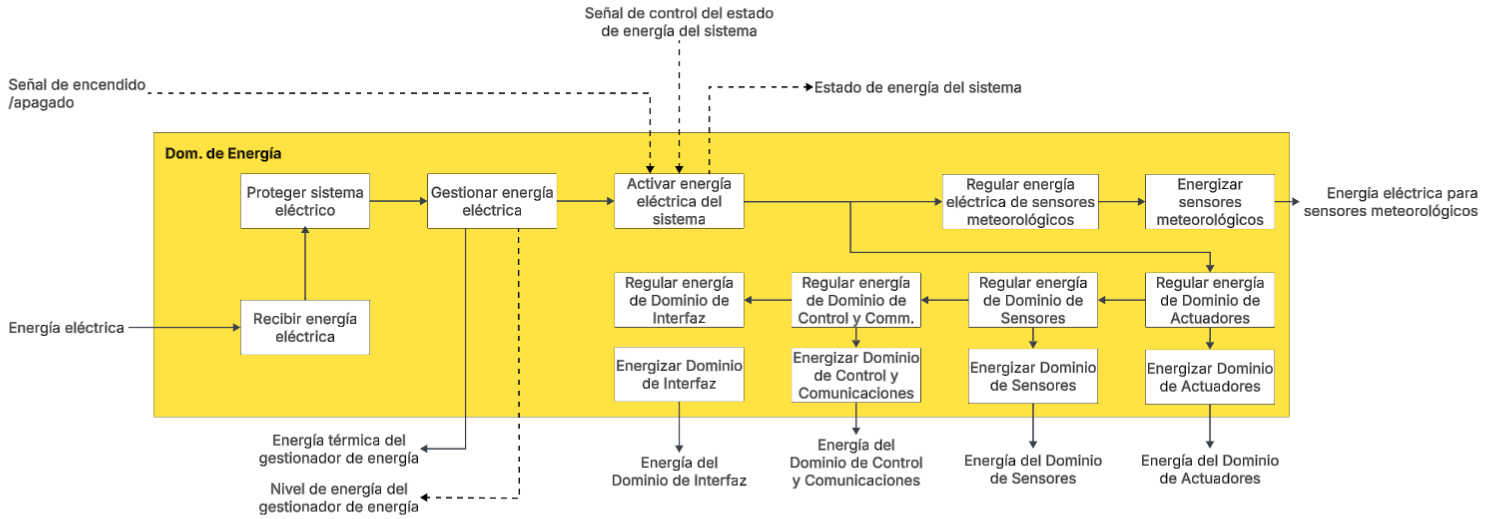
\includegraphics[width=1.2\textwidth]{Recursos/Imagenes/ImagenesDominios/A3_DominioEnergia.png}
	} \par\medskip
	
	\raggedright
	\footnotesize \textit{Nota.} Elaboración propia.
	\label{fig:Avance3_DomEnergia}
\end{figure}

\subsection{Dominio de Sensores}
El Dominio de Sensores actúa como el sistema de medición y detección del ambiente del robot, encargado de adquirir los estados físicos de los componentes y del entorno inmediato para su posterior procesamiento. Este dominio es alimentado de forma general por el flujo de energía del Dominio de Sensores. Está compuesto de las siguientes funciones, ilustaradas en la Figura \ref{fig:Avance3_DomSensores}:
\begin{enumerate}
	\item \textbf{Sensar temperatura de gestionador de energía:} Capta la energía térmica del gestionador de energía proveniente de dicho módulo y la traduce para emitir los datos brutos de temperatura del gestionador.
	\item \textbf{Sensar nivel de energía:} Lee el nivel de energía del gestionador de energía y lo convierte para entregar los datos brutos del nivel de energía del sistema.
	\item \textbf{Sensar presencia de obstáculo:} Detecta la presencia de obstáculos físicos en la ruta y devuelve la señal de obstáculo encontrado para alertar al control y garantizar su evasión.
	\item \textbf{Sensar velocidad de traslación:} Recibe físicamente la velocidad del mecanismo de traslación y proporciona retroalimentación emitiendo los datos brutos de velocidad.
	\item \textbf{Sensar orientación de plataforma:} Capta el grado de orientación de la plataforma y lo convierte en los datos brutos de orientación de la plataforma para permitir cerrar el lazo de control de la instrumentación.
	\item \textbf{Sensar posición de plataforma:} Recibe la posición de la plataforma física y emite los correspondientes datos brutos de posición de la plataforma.
	\item \textbf{Sensar orientación del sistema:} Capta la orientación del sistema global del vehículo y la transforma para entregar los datos brutos de orientación del sistema para la navegación espacial.
	\item \textbf{Captar señal GPS:} Recibe la señal GPS satelital externa y la devuelve como una señal GPS captada para posibilitar el seguimiento de rutas y geolocalización en el entorno.
\end{enumerate}

\begin{figure}[H]
	\captionsetup{justification=raggedright, singlelinecheck=false, labelsep=none}
	
	\caption[Dominio de sensores de la estructura de funciones.]{} 
	
	\textit{Dominio de sensores de la estructura de funciones.} \par\medskip
	
	\centering
	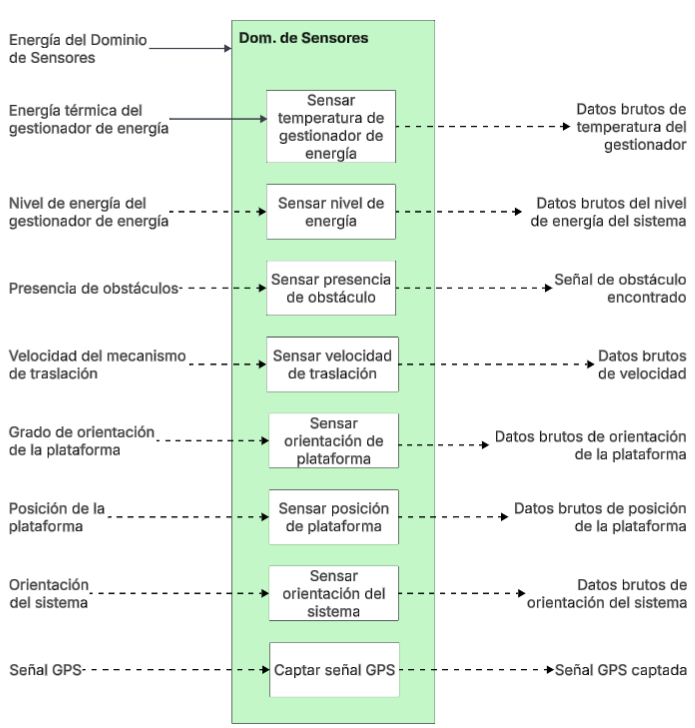
\includegraphics[width=0.8\textwidth]{Recursos/Imagenes/ImagenesDominios/A3_DominioSensores.png} \par\medskip
	
	\raggedright
	\footnotesize \textit{Nota.} Elaboración propia.
	\label{fig:Avance3_DomSensores}
\end{figure}
\subsection{Dominio de Control}

El Dominio de Control opera como el núcleo lógico y computacional del sistema, encargado de procesar la información recibida, gestionar la seguridad energética, registrar los datos climáticos y comandar tanto la navegación como los actuadores. Todo el subsistema es alimentado por la energía del Dominio de Control y el Dominio de Comunicaciones. Está compuesto de las siguientes funciones, vistas en la Figura \ref{fig:Avance3_DomControl}:

\begin{enumerate}
	\item \textbf{Procesar datos meteorológicos:} Recibe los datos meteorológicos brutos, enviándolos hacia el exterior como datos meteorológicos procesados y transfiriéndolos simultáneamente al bloque de registro.
	\item \textbf{Registrar datos meteorológicos:} Escribe la información recibida generando el flujo de comunicación con memoria externa de salida para el respaldo físico de los datos.
	\item \textbf{Procesar temperatura de gestionador:} Interpreta los datos brutos de temperatura del gestionador provenientes del módulo de energía.
	\item \textbf{Procesar nivel de energía:} Interpreta los datos brutos del nivel de energía del sistema y emite directamente la información sobre estado de energía hacia el exterior.
	\item \textbf{Procesar estado de energía del sistema:} Recibe y hace converger los flujos lógicos internos de temperatura y nivel de energía procesados para devolver una variable de estado general.
	\item \textbf{Controlar estado de energía del sistema:} Evalúa la variable del bloque anterior para generar la señal de control del estado de energía del sistema, la cual interactúa con el interruptor de encendido.
	\item \textbf{Procesar rutas de inspección:} Extrae la información espacial ingresada desde la comunicación con memoria externa de entrada para generar internamente la información procesada de rutas de inspección.
	\item \textbf{Procesar posición del sistema:} Interpreta los datos de posición del sistema brutos externos para derivar las coordenadas de posición del sistema.
	\item \textbf{Procesar presencia de obstáculo:} Evalúa la señal de obstáculo encontrado proveniente de los sensores, retransmitiéndola de forma directa como salida de alerta y generando internamente la posición de obstáculo.
	\item \textbf{Procesar orientación del sistema:} Recibe e interpreta los datos brutos de orientación del sistema para alimentar los cálculos de navegación espacial.
	\item \textbf{Procesar velocidad de traslación, procesar orientación de la plataforma y procesar posición de la plataforma:} Son tres funciones paralelas que interpretan de forma independiente los datos brutos de velocidad, los datos brutos de orientación de la plataforma y los datos brutos de posición de la plataforma, provenientes de la retroalimentación de los mecanismos físicos.
	\item \textbf{Controlar movimiento de actuador de traslación, orientación de plataforma y posicionamiento de plataforma):} Constituyen las tres etapas finales de salida de este dominio. Integran de forma conjunta las variables de navegación (rutas, coordenadas, orientación del sistema y obstáculos) con sus respectivos lazos de retroalimentación para emitir las señales de control respectivas.
\end{enumerate}

\begin{figure}[H]
	\captionsetup{justification=raggedright, singlelinecheck=false, labelsep=none}
	
	\caption[Dominio de control de la estructura de funciones.]{} 
	
	\textit{Dominio de control de la estructura de funciones.} \par\medskip
	
	\makebox[\textwidth][c]{ 
		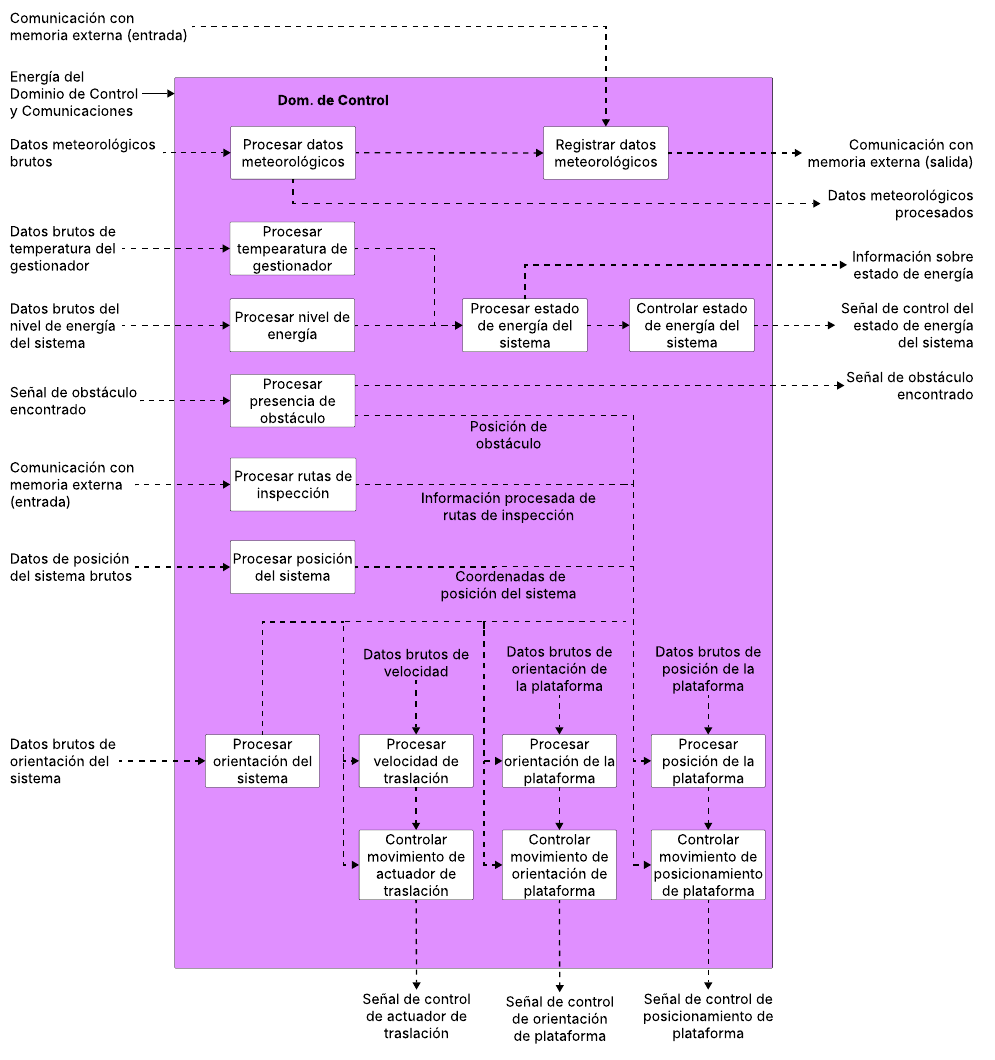
\includegraphics[width=0.9\textwidth]{Recursos/Imagenes/ImagenesDominios/A3_DominioControl.png}
	} \par\medskip
	
	\raggedright
	\footnotesize \textit{Nota.} Elaboración propia.
	\label{fig:Avance3_DomControl}
\end{figure}

\subsection{Dominio de Comunicación}

El Dominio de Comunicación actúa como el puente de telemetría entre el robot y la red externa del parque fotovoltaico. Para su operatividad, todo este subsistema se encuentra alimentado por el flujo de energía del Dominio de Control y el Dominio de Comunicaciones. El dominio se compone de las siguientes funciones, vistas en la Figura \ref{fig:Avance3_DomComunicacion}:

\begin{enumerate}
	\item \textbf{Procesar señal GPS recibida:} Capta e interpreta la señal de radiofrecuencia satelital proveniente del entorno para transformarla y entregar los datos de posición del sistema brutos, los cuales son requeridos por la lógica de navegación interna.
	
	\item \textbf{Procesar señal de mando recibida:} Gestiona el enlace interactivo de entrada proveniente de la señal de control de telecomunicación. Principalmente, esta función decodifica la trama de los comandos de telemetría, asegurando una respuesta inmediata del robot frente a instrucciones del usuario.
	
	\item \textbf{Transmitir estado telemétrico:} Emite la señal de estado de transmisión telemétrica hacia el exterior, lo que permite a la estación base monitorear de forma continua la calidad, latencia e integridad del enlace de red con el vehículo.
	
	\item \textbf{Transmitir datos meteorológicos:} Constituye la etapa final del reporte climático y operativo. Esta función recibe los datos meteorológicos procesados desde el dominio de control, y seguidamente codifica y empaqueta la información en un payload para enviarla hacia la estación base en forma de paquetes de datos meteorológicos consolidados.
\end{enumerate}

\begin{figure}[H]
	\captionsetup{justification=raggedright, singlelinecheck=false, labelsep=none}
	
	\caption[Dominio de comunicaciones de la estructura de funciones.]{} 
	
	\textit{Dominio de comunicaciones de la estructura de funciones.} \par\medskip
	
	\makebox[\textwidth][c]{ 
		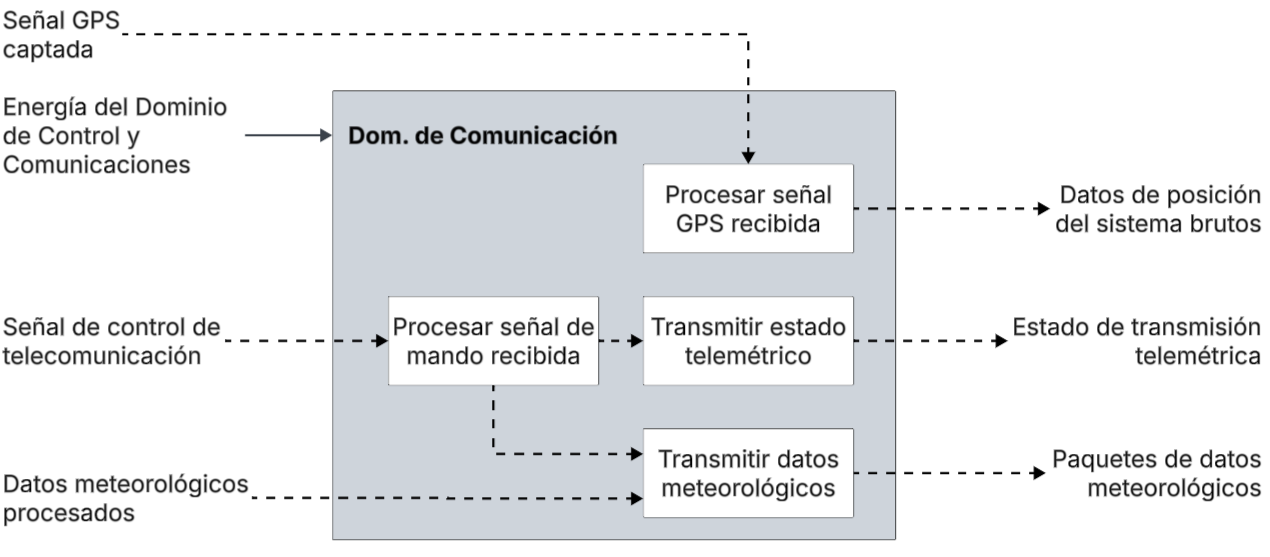
\includegraphics[width=0.8\textwidth]{Recursos/Imagenes/ImagenesDominios/A3_DominioComunicacion.png}
	} \par\medskip
	
	\raggedright
	\footnotesize \textit{Nota.} Elaboración propia.
	\label{fig:Avance3_DomComunicacion}
\end{figure}

\subsection{Dominio de Interfaz}

El Dominio de Interfaz, mostrado en la Figura \ref{fig:Avance3_DomInterfaz}  desempeña un rol dual en la arquitectura del robot: por un lado, actúa como el puerto de conexión para la instrumentación climática periférica y, por otro, se encarga de exteriorizar los estados operativos y advertencias críticas hacia el personal en el parque fotovoltaico. Para su funcionamiento general, todos los componentes de este subsistema son alimentados directamente por el flujo de energía del Dominio de Interfaz. El dominio cuenta con los siguientes bloques de función:

\begin{enumerate}
	\item \textbf{Accionar movimiento de traslación:} Recibe la señal de control del actuador de traslación y la transforma en la energía cinética necesaria para ejecutar el desplazamiento principal del robot.
	\item \textbf{Accionar movimiento de orientación de plataforma:} Procesa la señal de control de orientación y genera la energía cinética correspondiente para ajustar este parámetro en la plataforma de medición.
	\item \textbf{Accionar movimiento de posicionamiento de plataforma:} Recibe la señal de control de posicionamiento y la convierte en la energía cinética requerida para el ajuste físico final de la plataforma.
\end{enumerate}

\begin{figure}[H]
	\captionsetup{justification=raggedright, singlelinecheck=false, labelsep=none}
	
	\caption[Dominio de interfaz de la estructura de funciones.]{} 
	
	\textit{Dominio de interfaz de la estructura de funciones.} \par\medskip
	
	\makebox[\textwidth][c]{ 
		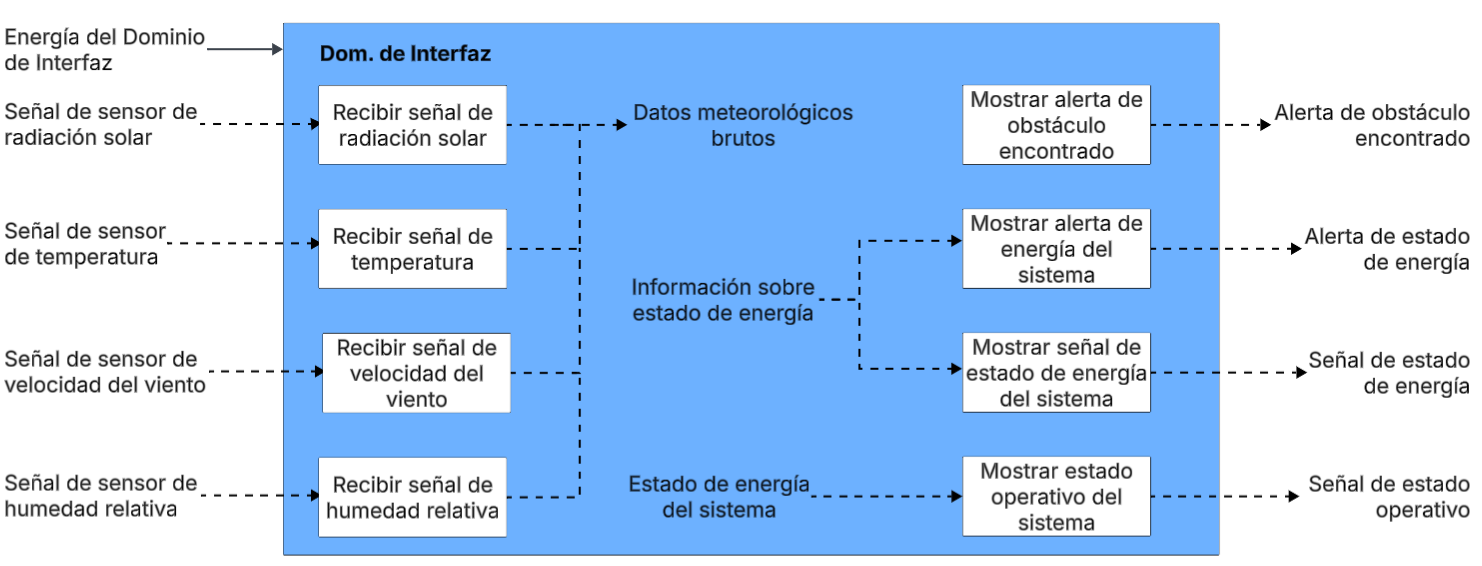
\includegraphics[width=1.0\textwidth]{Recursos/Imagenes/ImagenesDominios/A3_DominioInterfaz.png}
	} \par\medskip
	
	\raggedright
	\footnotesize \textit{Nota.} Elaboración propia.
	\label{fig:Avance3_DomInterfaz}
\end{figure}

\subsection{Dominio de Actuadores}
El Dominio de Actuadores, mostrado en la Figura \ref{fig:Avance3_DomActuadores}, es el encargado de transformar la energía eléctrica y las instrucciones lógicas en los esfuerzos cinéticos necesarios para la operación física del robot y el ajuste de sus instrumentos. Para su funcionamiento general, todo este subsistema es alimentado por el flujo de energía del Dominio de Actuadores. El dominio se compone de las siguientes funciones:

\begin{enumerate}
	\item \textbf{Accionar movimiento de traslación:} Recibe la señal de control del actuador de traslación y la transforma en la energía cinética necesaria para ejecutar el desplazamiento principal del robot.
	\item \textbf{Accionar movimiento de orientación de plataforma:} Procesa la señal de control de orientación y genera la energía cinética correspondiente para ajustar este parámetro en la plataforma de medición.
	\item \textbf{Accionar movimiento de posicionamiento de plataforma:} Recibe la señal de control de posicionamiento y la convierte en la energía cinética requerida para el ajuste físico final de la plataforma.
\end{enumerate}

\begin{figure}[H]
	\captionsetup{justification=raggedright, singlelinecheck=false, labelsep=none}
	
	\caption[Dominio de actuadores de la estructura de funciones.]{} 
	
	\textit{Dominio de actuadores de la estructura de funciones.} \par\medskip
	
	\centering
	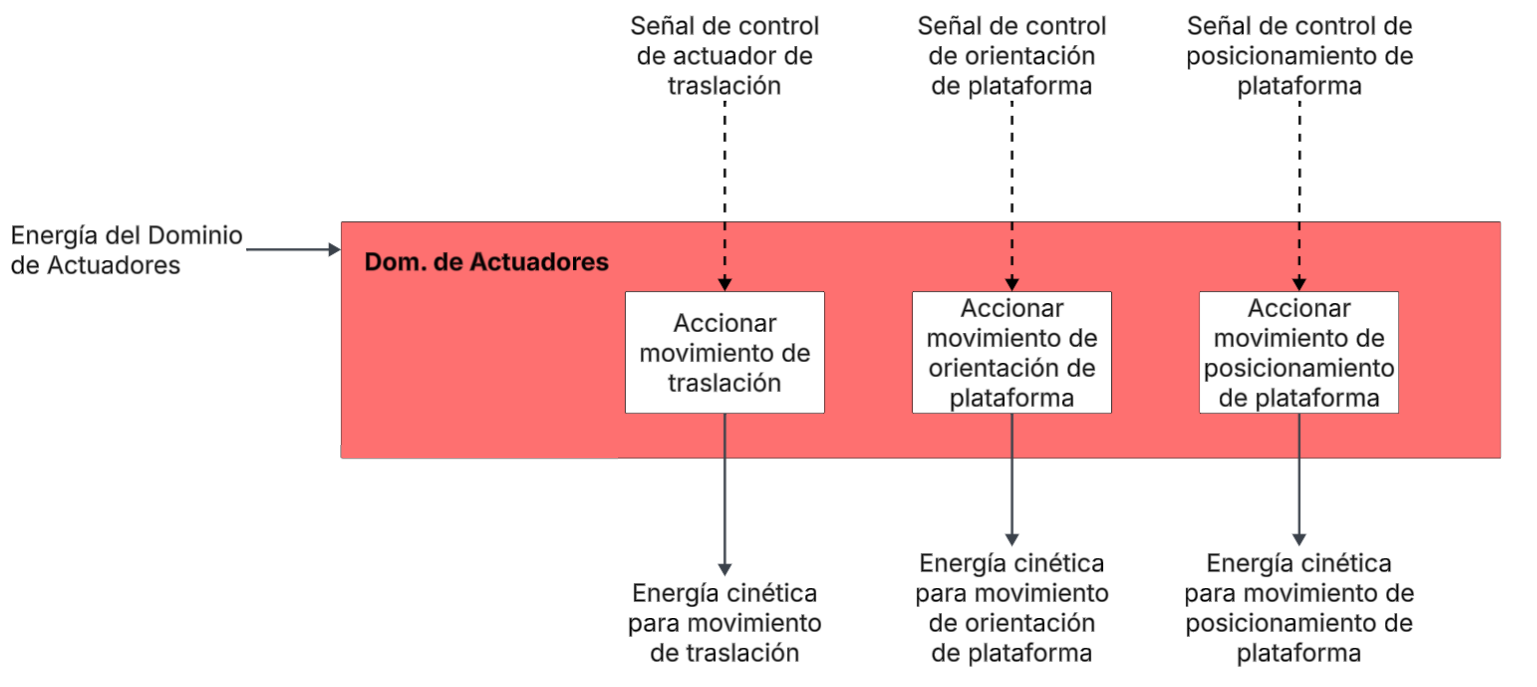
\includegraphics[width=0.99\textwidth]{Recursos/Imagenes/ImagenesDominios/A3_DominioActuadores.png} \par\medskip
	
	\raggedright
	\footnotesize \textit{Nota.} Elaboración propia.
	\label{fig:Avance3_DomActuadores}
\end{figure}

\subsection{Dominio Mecánico}

El Dominio Mecánico, mostrado en la Figura \ref{fig:Avance3_DomMecanico}, conforma el soporte estructural del vehículo y materializa las interacciones dinámicas y físicas con el entorno del parque solar. Está compuesto de las siguientes funciones:

\begin{enumerate}
	\item \textbf{Soportar plataforma de medición de radiación:} Sostiene la carga física de la instrumentación climática frente a las vibraciones mecánicas del entorno.
	\item \textbf{Proteger componentes internos:} Aísla el equipo para garantizar la integridad de la tecnología frente a factores externos como la suciedad del ambiente.
	\item \textbf{Soportar componentes:} Provee la base física unificada y el soporte estructural estático general para el resto del sistema.
	\item \textbf{Alojar gestionador de energía:} Provee la contención estructural física específica para el gestionador del sistema de energía.
	\item \textbf{Alojar memoria externa:} Actúa como la interfaz material que recibe la memoria externa física. Transmite la comunicación de entrada (rutas de inspección y formatos) al control y recibe la señal de salida para grabar los datos registrados.
	\item \textbf{Generar movimiento de traslación:} Transforma la energía cinética recibida en el desplazamiento general sobre el terreno, retroalimentando al sistema con la velocidad del mecanismo de traslación.
	\item \textbf{Orientar plataforma de medición de radiación:} Utiliza la energía cinética proveniente de los actuadores para ejecutar el cambio de ángulo, entregando como información el grado de orientación de la plataforma.
	\item \textbf{Posicionar plataforma de medición de radiación:} Emplea la energía cinética correspondiente para su ajuste espacial final, suministrando la posición de la plataforma para cerrar los lazos de control y generando las vibraciones emitidas hacia el exterior.
\end{enumerate}
\begin{figure}[H]
	\captionsetup{justification=raggedright, singlelinecheck=false, labelsep=none}
	
	\caption[Dominio mecánico de la estructura de funciones.]{} 
	
	\textit{Dominio mecánico de la estructura de funciones.} \par\medskip
	
	\makebox[\textwidth][c]{ 
		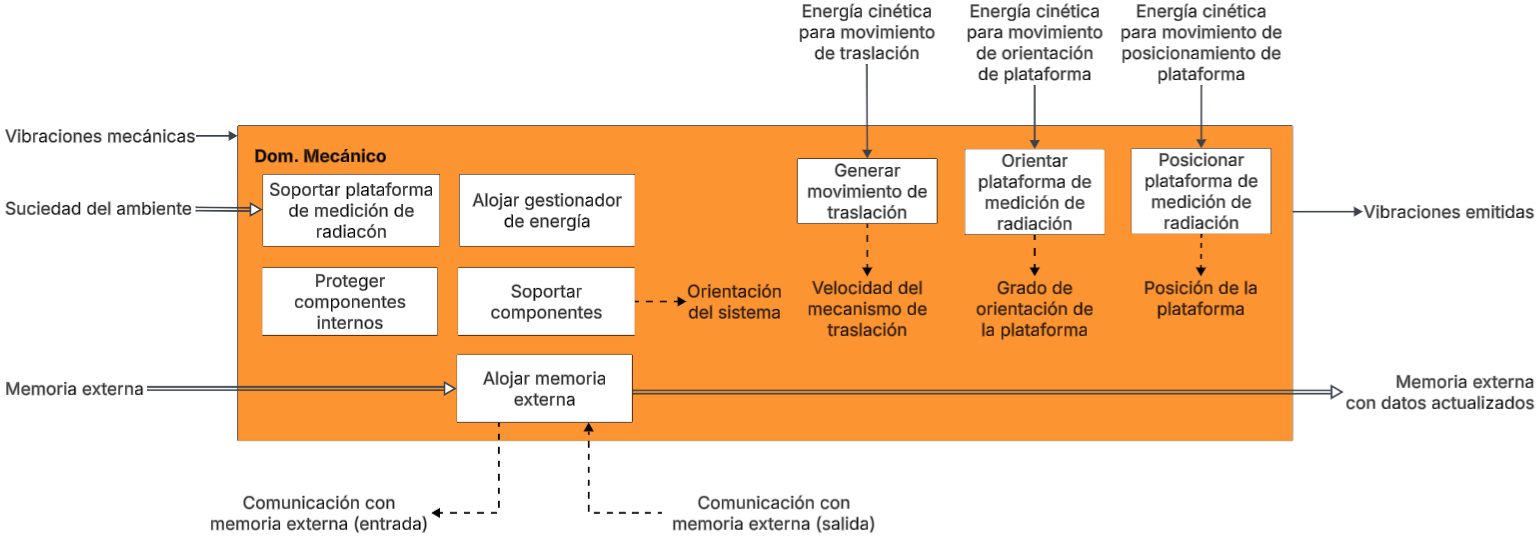
\includegraphics[width=1.25\textwidth]{Recursos/Imagenes/ImagenesDominios/A3_DominioMecanico.png}
	} \par\medskip
	
	\raggedright
	\footnotesize \textit{Nota.} Elaboración propia.
	\label{fig:Avance3_DomMecanico}
\end{figure}

\end{document}